\section{Introduction à la blockchain}
\framewithtitle{Introduction à la blockchain}

\begin{frame}{Sommaire}
  \setcounter{tocdepth}{2}
  \tableofcontents[currentsection, hideothersubsections]
\end{frame}


\begin{frame}{Objectifs de ce module}
  \begin{enumerate}
    \item Comprendre les enjeux basiques de la blockchain
    \item Développer des smart-contracts de tokens fongibles et non-fongibles
    \item Se sensibiliser à la sécurité de la blockchain
  \end{enumerate}
\end{frame}

\subsection{Définitions générales}
\framewithtitle{Définitions générales}

\begin{frame}{Contexte historique : origines de la blockchain}
  \begin{itemize}
    \item 2008 : Satoshi Nakamoto publie \href{https://bitcoin.org/bitcoin.pdf}{\textquote{Bitcoin: A Peer-to-Peer Electronic Cash System}}
    \item Dans ces neuf pages, Nakamoto décris un système financier et introduit les bases de la blockchain
          \begin{itemize}
            \item Structure en blocs
            \item Cryptographie (hachage, asymmétrique, arbres de Merkel...)
            \item Transactions
          \end{itemize}
    \item Fun fact : Satoshi Nakamoto est toujours resté anonyme
  \end{itemize}
\end{frame}

\begin{frame}{Définition générale}
  Blockchain se traduit par \textquote{chaîne de blocs}.
  Il s'agit donc d'un système permettant de stocker et de partager de l'information au travers d'un \textbf{structure de données bien choisie construite à partir de plusieurs blocs} (et c'est tout).

  La majorité des systèmes de blockchain possèdent des caractéristiques supplémentaires qui sont utilisées par abus de langage :

  \begin{enumerate}
    \item Présence d'une cryptomonnaie liée à la blockchain (il existe des blockchains SANS cryptomonnaies)
    \item Décentralisation
    \item Autonome/sans administration centrale
    \item Anonymat/pseudonimat des utilisateurs
  \end{enumerate}
\end{frame}

\begin{frame}{Définitions tierces}
  economie.gouv.fr
  \begin{quote}
    Développée à partir de 2008, c'est, en premier lieu, une technologie de stockage et de transmission d’informations. Cette technologie offre de hauts standards de transparence et de sécurité car elle fonctionne sans organe central de contrôle.

    Plus concrètement, la chaîne de blocs permet à ses utilisateurs - connectés en réseau - de partager des données sans intermédiaire.
  \end{quote}


  Wikipédia
  \begin{quote}
    Une blockchain, ou chaîne de blocs, est une technologie de stockage et de transmission d'informations sans autorité centrale. Techniquement, il s'agit d'une base de données distribuée dont les informations envoyées par les utilisateurs et les liens internes à la base sont vérifiés et groupés à intervalles de temps réguliers en blocs, formant ainsi une chaîne.
  \end{quote}
\end{frame}


\subsection{Cryptographie}
\framewithtitle{Cryptographie}

\begin{frame}{Notations}
  \begin{tiny}
    \textit{Je suis désolé, il faut faire un tout petit peu de maths...}
  \end{tiny}

  Dans la suite, je vais noter :

  \begin{itemize}
    \item $\mathbb{B} = \{0,1\}^\mathbb{N}$ l'ensemble des mots binaires
    \item $\mathbb{B}_{n \in \mathbb{N}} = \{0,1\}^n$ l'ensemble des mots binaires de taille $n$
  \end{itemize}

  Exemples :

  \begin{itemize}
    \item $B_3 = \{000, 001, 010, 011, 100, 101, 110, 111\}$
    \item $010010$ est un mot binaire de 6 bits, il est donc membre de $\mathbb{B}_6$
  \end{itemize}
\end{frame}

\begin{frame}{Qu'est-ce que la cryptographie ?}
  \begin{columns}
    \begin{column}{0.65\textwidth}
      TL;DR = utiliser les mathématiques au service de la sécurité de l'information

      Exemples historiques :
      \begin{itemize}
        \item Chiffrement de César : décalage de lettre de 1 à 25
        \item Chiffrement de Vigenère : sustitions de lettres à partir d'une clé secrète
        \item Chiffrement affine : subsutition de lettre à l'aide d'une équation affine
        \item Enigma (seconde guerre modiale) : machine de chiffrement allemande
      \end{itemize}
    \end{column}

    \begin{column}{0.3\textwidth}
      \begin{figure}
  \resizebox{\textwidth}{!}{
    \includegraphics{img/enigma.png}
  }

  \caption{Machine Enigma}
  \label{fig:enigma}
\end{figure}
    \end{column}
  \end{columns}
\end{frame}

\subsubsection{Hachage}
\begin{frame}{Somme de contrôle : définition}
  \begin{definition}
    Une somme de contrôle est une petite quantité de données additionnelle qui est calculée à partir d'un ensemble plus large de données. Elle est utilisée pour vérifier l'intégrité des données et détecter les erreurs ou les altérations éventuelles.
  \end{definition}
\end{frame}

\begin{frame}[fragile]{Somme de contrôle : exemple du numéro de sécurité sociale}
  Les deux derniers chiffre du numéro de sécurité sociale ne contiennent aucune information mais ils sont utilisés comme somme contrôle, pour limiter les risques de faute d'erreur.

  La formule permettant de calculer la clé est la suivante :

  $$
    \textrm{clé} = 97 - NIR \bmod 97
  $$

  Prenons l'exemple suivant :

  $$
    \underbrace{2 69 05 49 588 157}_{\textrm{numéro NIR}}\underbrace{80}_{\textrm{clé}}
  $$

  \begin{minted}{text}
    >>> 97 - 2690549588157 % 97
    80
  \end{minted}
\end{frame}

\begin{frame}{Fonction de hachage : définition}
  \begin{columns}
    \begin{column}{0.7\textwidth}
      Comment appliquer cette logique à de l'information binaire ?
      On cherche une somme de contrôle universelle capable de fonctionner sur tout $\mathbb{B}$.

      $\Rightarrow$ on les appelle fonction de hachage

      \begin{definition}
        Une fonction de hachage permet de générer un \textquote{hash} de n'importe quel mot binaire.
      \end{definition}

      \begin{definition}
        Un hash est un mot binaire de taille fixe, dont la taille est spécifique à la fonction de hachahe utilisé.
      \end{definition}
    \end{column}
    \begin{column}{0.2\textwidth}
      \resizebox{\textwidth}{!}{
        \includegraphics{img/meat-grinder.png}
      }
    \end{column}
  \end{columns}
\end{frame}

\begin{frame}[fragile]{Fonction de hachage : exemples}
  \begin{minted}{text}
    >>> import hashlib
    >>> hashlib.sha256(b"Mathieu").hexdigest()
    'f5e088d29801ebb822251d7751bc4b8ff28c50132d8b0a95614b5f048a1d01b6'
  \end{minted}

  \begin{figure}
  \resizebox{\columnwidth}{!}{%
    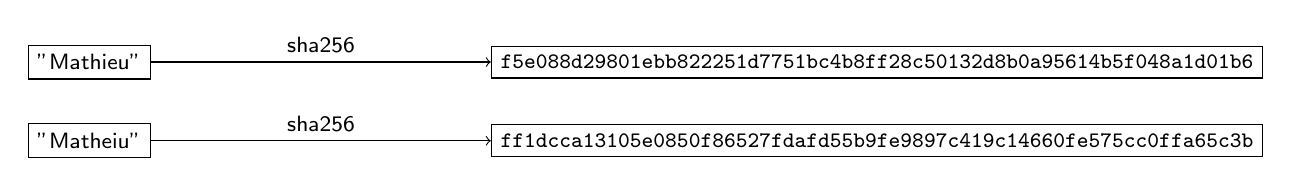
\begin{tikzpicture}[font=\sffamily\footnotesize,
        Input/.style={shape=rectangle,draw},
        Output/.style={shape=rectangle,draw}
      ]

      \node[Input] (I_1) at (0,0) {"Mathieu"};
      \node[Output] (O_1) at (10,0) {\texttt{f5e088d29801ebb822251d7751bc4b8ff28c50132d8b0a95614b5f048a1d01b6}};
      \node[Input] (I_2) at (0,-1) {"Matheiu"};
      \node[Output] (O_2) at (10,-1) {\texttt{ff1dcca13105e0850f86527fdafd55b9fe9897c419c14660fe575cc0ffa65c3b}};

      \draw[->] (I_1) -- (O_1) node[midway,above,sloped]{sha256};
      \draw[->] (I_2) -- (O_2) node[midway,above,sloped]{sha256};
    \end{tikzpicture}%
  }

  \caption{Hachage avec SHA-256}
  \label{fig:sha256-hash-examples}
\end{figure}
\end{frame}

\begin{frame}{Caractéristiques d'une fonction de hachage}
  \begin{block}{Collision}
    Une fonction de hachage $h$ de taille $n$ entraîne obligatoirement des collisions car la taille de $\mathbb{B}$ est infinie alors que $\mathbb{B}_n$ n'est \textquote{que} de $2^n$.
    Une collision existe quand deux mots binaires $a$ et $b$ engendrent le même hash, c'est-à-dire :

    $$h(a) = h(b)$$

    $\Rightarrow$ une \textquote{bonne} fonction de hachage ne possède pas de hash connu.
  \end{block}

  Les alorithme md4, md5 et sha1 ne sont à jour plus considérés comme sûrs.
\end{frame}

\subsubsection{Chiffrement symétrique}
\subsubsection{Chiffrement asymétrique}
\subsubsection{Signature digitale}


\subsection{Exemple du Bitcoin}
\framewithtitle{Exemple du Bitcoin}
\begin{frame}{Centralisation}
  Exemples:

  \begin{enumerate}
    \item L'Euro: la banque centrale européenne est souveraine et peut émettre des euros
    \item La force nucléaire en France : contrôlée par l'armée
    \item Twitter : la direction peut décider de retirer des privilèges sans l'approbation des utilisateurs (arrivée d'Elon Musk...)
  \end{enumerate}

  \begin{itemize}
    \item[$\Rightarrow$] La centralisation place un privilège/pouvoir entre les mains d'un petit groupe
    \item[$\Rightarrow$] Inversement, les utilisateurs sont tributaire du bon vouloir/bon fonctionement des systèmes
    \item[$\Rightarrow$] Une relation de \textbf{confiance} est nécessaire
  \end{itemize}
\end{frame}

\begin{frame}{Bitcoin : décentralisation}
  \begin{columns}
    \begin{column}{0.6\textwidth}
      \begin{itemize}
        \item La blockchain Bitcoin est un réseau peer-to-peer décentralisé
        \item Le réseau Bitcoin \textbf{toujours en ligne} (tant qu'il y a des noeuds)
        \item Pas d'administration centrale (donc pas de Bitcoin Corp. Limited)
        \item Tout individu peut y participer en créant un \textquote{n\oe{}ud} = démarrer un logiciel en CLI
      \end{itemize}
    \end{column}

    \begin{column}{0.4\textwidth}
      \begin{figure}
  \resizebox{\columnwidth}{!}{%
    \begin{tikzpicture}[font=\sffamily\footnotesize,
        Node/.style={shape=ellipse,draw}
      ]

      \node[Node] (N_A) at (0,0) {Node A};
      \node[Node, above right=2cm and 2cm of N_A] (N_B) {Node B};
      \node[Node, below right=2cm and 2cm of N_A] (N_C) {Node C};
      \node[Node, above left=2cm and 2cm of N_A] (N_D) {Node D};
      \node[Node, below left=2cm and 2cm of N_A] (N_E) {Node E};

      \draw[<->] (N_A) -- (N_B);
      \draw[<->] (N_A) -- (N_C);
      \draw[<->] (N_A) -- (N_D);
      \draw[<->] (N_A) -- (N_E);
      \draw[<->] (N_D) -- (N_E);
      \draw[<->] (N_D) -- (N_B);
      \draw[<->] (N_C) -- (N_E);
      \draw[<->] (N_C) -- (N_B);
    \end{tikzpicture}%
  }

  \caption{Réseau peer-to-peer}
\end{figure}
    \end{column}
  \end{columns}
\end{frame}

\begin{frame}[fragile]{Bitcoin : livre de comptes}
  \begin{columns}
    \begin{column}{0.05\textwidth}
    \end{column}

    \begin{column}{0.65\textwidth}
      La blockchain Bitcoin est un système décentralisé permettant aux utilisateurs d'échanger une monnaie numérique, le Bitcoin.

      \begin{itemize}
        \item Les Bitcoin (BTC) sont stockés dans des comptes, identifiés par une adresse
        \item L'ensemble des soldes des comptes, le \textquote{livre de comptes} est stocké à de multiples endroits
        \item Tout individu peut obtenir un compte gratuitement (on en parle plus tard)
        \item Envoyer des $x$ BTC d'une adresse $a$ à une adresse $b$ revient à faire
      \end{itemize}

      \begin{minted}{solidity}
        solde_a -= x
        solde_b += x
      \end{minted}
    \end{column}

    \begin{column}{0.2\textwidth}
      \begin{table}[]
  \begin{tabularx}{\textwidth}{X|l}
    \toprule
    Compte & Solde \\ \midrule
    0001   & 12    \\
    0002   & 3.42  \\
    0003   & 4.4   \\
    0004   & 3.6   \\
    0005   & 5     \\
    \vdots &       \\
    1232   & 30.45 \\
    1233   & 0.34  \\
    1234   & 113.3 \\
    1235   & 4.97  \\ \bottomrule
  \end{tabularx}
\end{table}
    \end{column}

    \begin{column}{0.1\textwidth}
    \end{column}
  \end{columns}
\end{frame}

\begin{frame}{Bitcoin : opérer un node}
  \begin{columns}
    \begin{column}{0.5\textwidth}
      \begin{itemize}
        \item Opérer un node = particper à la blockchain = augmenter la décentralisation
        \item \textquote{Relativement léger} : 2 Go de RAM, 7 Go de disque, connexion 400 kilobits/sec
        \item Attention, certains pays interdisent d'opérer un node : Afghanistan, Algérie, Bangladesh, Bolivie, Chine, Égypte, Kosovo, Maroc, Népal
      \end{itemize}
    \end{column}

    \begin{column}{0.5\textwidth}
      \begin{figure}
  \resizebox{\textwidth}{!}{
    \includegraphics{img/btc-core-gui.png}
  }
  \caption{Bitcoin Core GUI}
  \label{fig:btc-core-gui}
\end{figure}
    \end{column}
  \end{columns}
\end{frame}

\subsection{Blockchain}

\subsection{Problème du consensus}
\subsubsection{Proof of work}
\subsubsection{Proof of stack}

\framewithtitle{Blockchain}